\chapter{Literature Review}
This final project discusses the design model to determining k-nearest emergency unit from emergency location. To establish the groundwork, this chapter will discuss theories and facts related.

\section{Emergency}
Emergency is an abnormal event that have negative impact. It can threaten and disrupt a person's life. An emergency can be presented in many forms; from everyday incidents like traffic accident or assault, to major incidents like wildfire, earthquake, or large-scale terrorist attacks. Emergency occurs suddenly with unexpected place and time \cite{hauke2011}.

\subsection{Emergency Services}

Emergency services ensure public safety by addressing emergency location and doing first aid. Basically there are three main emergency service functions which are law enforcement, emergency medical services, and fire service. These three function works as one and managed by emergency center. 

Emergency services vary widely in their use of technology. In some country, emergency services are reached by calling desired service by calling 7-digit telephone number, and then contacting the agency directly. In other areas, technology allows callers to use the single telephone number for every service they want.


\begin{figure}[H]
    \centering
    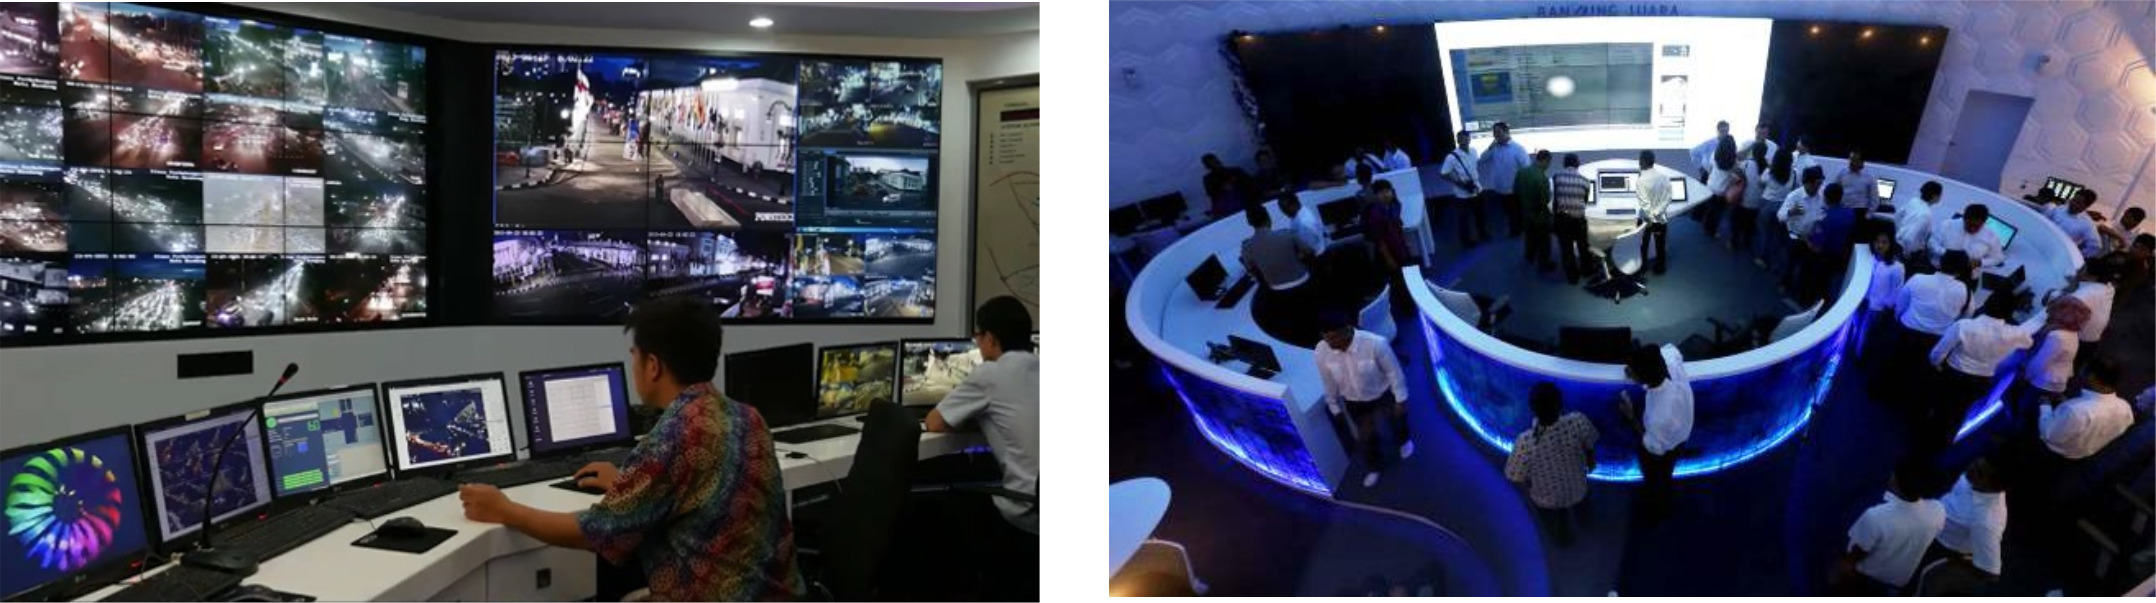
\includegraphics[scale=0.7]{emergency_center.png}
    \caption{Emergency Service Center in Bandung}
    \label{fig:emergency-units}
\end{figure}


\pagebreak
\subsection{Emergency Units}
Emergency unit is any unit that has to respond to an emergency in a life-threatening situation. In some major countries, the emergency unit consists of ambulance, police, and fire brigade. These units dispatched from a centre that takes calls from an emergency request. 

Many emergency units are likely to be fitted with audible and visual warning devices, which are designed to facilitate their movement through traffic to reach their destination, and to provide some protection on the scene. Traditionally, these units have relied on experience, practiced skills, good equipment, and teamwork for effective and successful emergency response.

\begin{figure}[H]
    \centering
    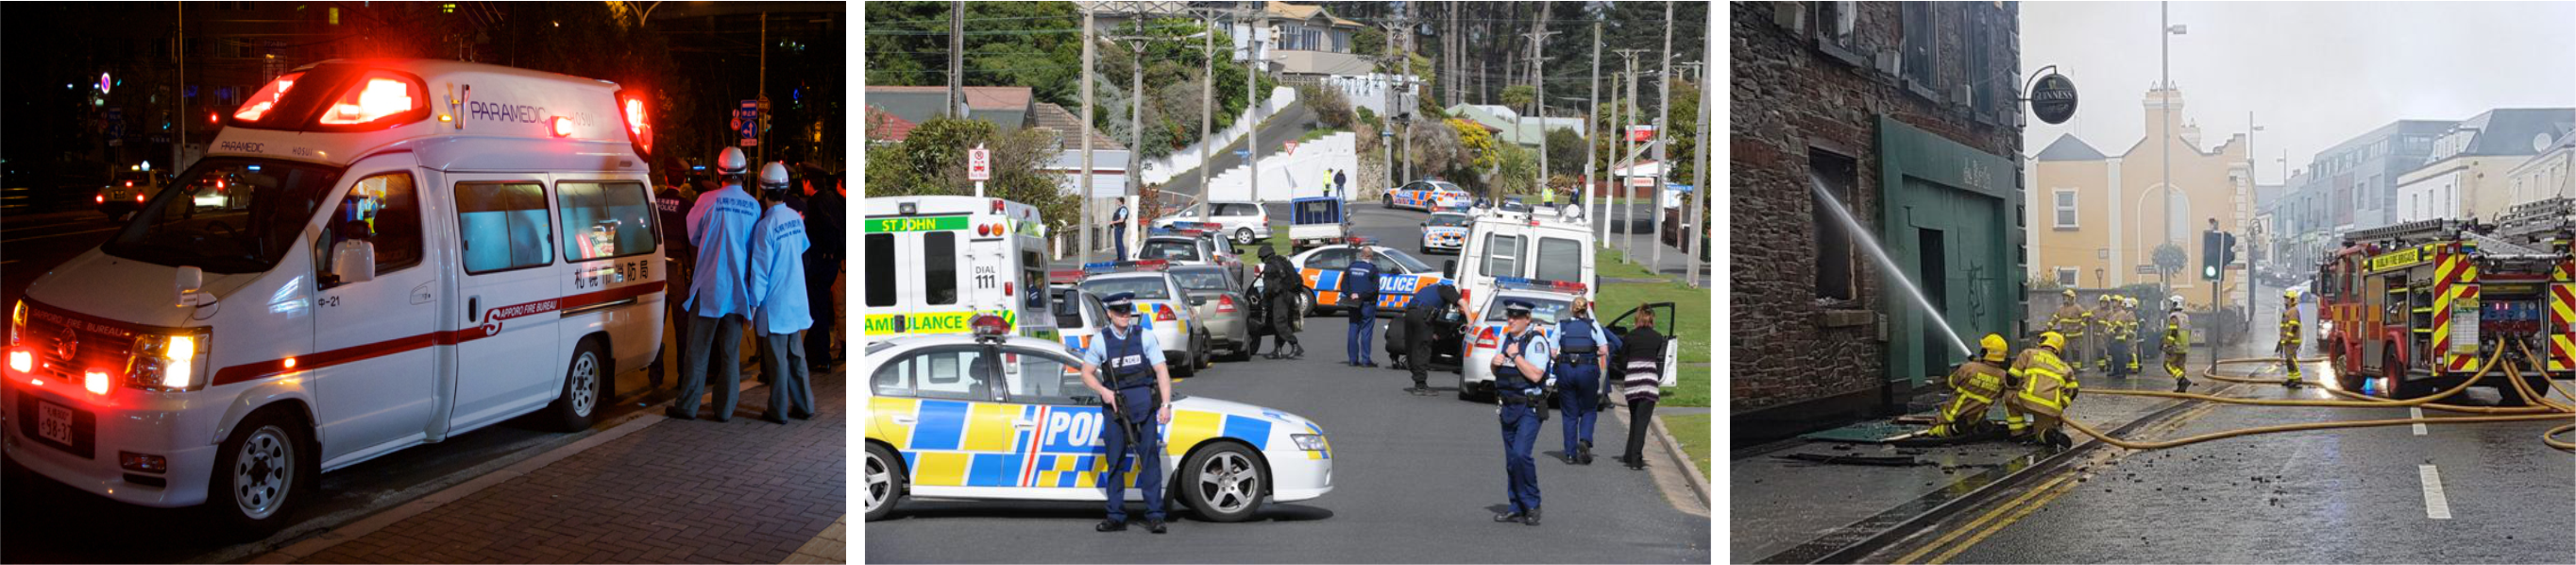
\includegraphics[scale=0.6]{emergency-units.png}
    \caption{Emergency Units consist of ambulance, police, and fire brigade}
    \label{fig:emergency-units}
\end{figure}

\section{Geographic Information System}
A GIS is required to monitor environmental conditions for various applications including policy making. This involves the use of data. A GIS will, in general, have a means of inputting data into a database, editing the data, displaying information stored in the database, and performing certain calculations including sorting of the data in the database. The nature of the data stored and the analytical and modeling capacity of a GIS will determine the solution to particular problems related to floods or land use planning or other potential needs \cite{ondieki1997}.

The role of a GIS is to enable the capture, storage, and manipulation of data in a structured form, therefore allowing the use of analytical techniques on the spatial dimensions of problems. With a GIS, analysis and depiction of spatially referenced information as well as dissemination of results of analysis using thematic maps is possible. Environmental science and other disciplines have generated enormous amounts of data of many different types, and this is bound to increase in future \cite{raju1997}.

\pagebreak
\subsection{Spatial Data}

In various fields there is a need to manage geometric, geographic, or spatial data, which means data related to space.  While typical databases have developed to manage various numeric and character types of data, such databases require additional functionality to process spatial data types efficiently, and developers have often added geometry or feature data types \cite{ooi1993}.

Spatial database is data that has, as a property, some connection with coordinates in a 2-dimensional, 3-dimensional space or even a higher dimensional space. Spatial data are large in quantity and are complex in structures and relationships. Spatial data properties shown as follows \cite{bonham-carter2014} :
\begin{enumerate}[leftmargin=*, topsep=5pt, itemsep=-1ex, partopsep=1ex, parsep=2ex]
\item Spatial Data Types: \\ It should support the point, line and surface types, since in daily practice people are familiar with the use of these objects.
\item Data Structures: \\ They should be simple. As opposed to the First Normal Form (1NN) relational model, for example, it is noticed that a nested model, though more powerful, is more difficult to both implement and use. Similarly, it is penalizing for the user to process two distinct data structures.
\item Spatial Operations: \\ They should apply to structures containing any type of spatial data.
\end{enumerate}

\begin{figure}[H]
    \centering
    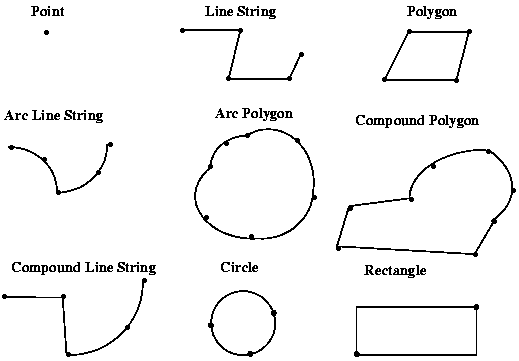
\includegraphics[scale=0.6]{spatial_data.png}
    \caption{Spatial Data Types}
    \label{fig:gis}
\end{figure}


\pagebreak
\subsection{Map Overlay}
The map overlay operation is a building block for various analysis operations in GIS. Its involves unions or intersection for two-map overlay. Map overlay works by executed as a sequence if binary map overlay operations. Map overlay implemented in either vector or raster system. In the vector case, often referred to as polygon overlay, the intersection of two or more data layers produces new features (polygons). Attributes (symbolized as colors in the illustration) of intersecting polygons are combined. The raster implementation (known as grid overlay) combines attributes within grid cells that align exactly. Misaligned grids must be resampled to common formats \cite{jampani2004}.

\begin{figure}[H]
    \centering
    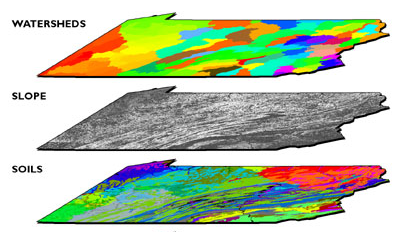
\includegraphics[scale=0.8]{map_overlay.png}
    \caption{map overlay illustration}
    \label{fig:gis}
\end{figure}


\section{Optimization Problems}
Optimization is the search for the values of variables that are considered optimal, effective, and efficient to achieve the desired goals. The optimization problem varies according to the conditions under which the system works. One of the most frequent optimization problems especially in the field of transportation is the search for the shortest path \cite{hannawati2002}.

Optimization in the shortest path can be based on the nearest distance to a facility or based on the fastest time to achieve it. This settlement process should still take into account the conditions that arise in it for a journey from the origin to the destination point such as traffic jam. The result of solving the shortest route problem can be called an optimal route. The optimal route is a route that has minimum travel time and distance.

\subsection{Solution of Optimization Problems}
To solving the problem of finding the shortest path can be done by using two methods, namely conventional method and heuristic method. Conventional methods are applied with ordinary mathematical calculations, while heuristic methods are applied with artificial intelligence calculations \cite{mutakhiroh2007}.
\pagebreak
\begin{enumerate}
\item The conventional method is a method that uses ordinary mathematical calculations. There are several conventional methods commonly used to perform the shortest path search, including: djikstra algorithm, Floyd-Warshall algorithm, and Bellman-Ford algorithm.

\item The heuristic method is a sub-field of artificial intelligence used for search and optimization. There are several algorithms on heuristic methods commonly used in optimization problems, including genetic algorithms, ant algorithms, fuzzy logic, neural networks, taboo search, simulated annealing, and others.
\end{enumerate}

\subsection{Solution of Shortest Path Problems}
The shortest path is a travel routing network in which a road steer wants to determine the shortest path between two cities, based on some available alternative paths, where the destination point is only one. The case can be illustrated as follows :

\begin{figure}[H]
    \centering
    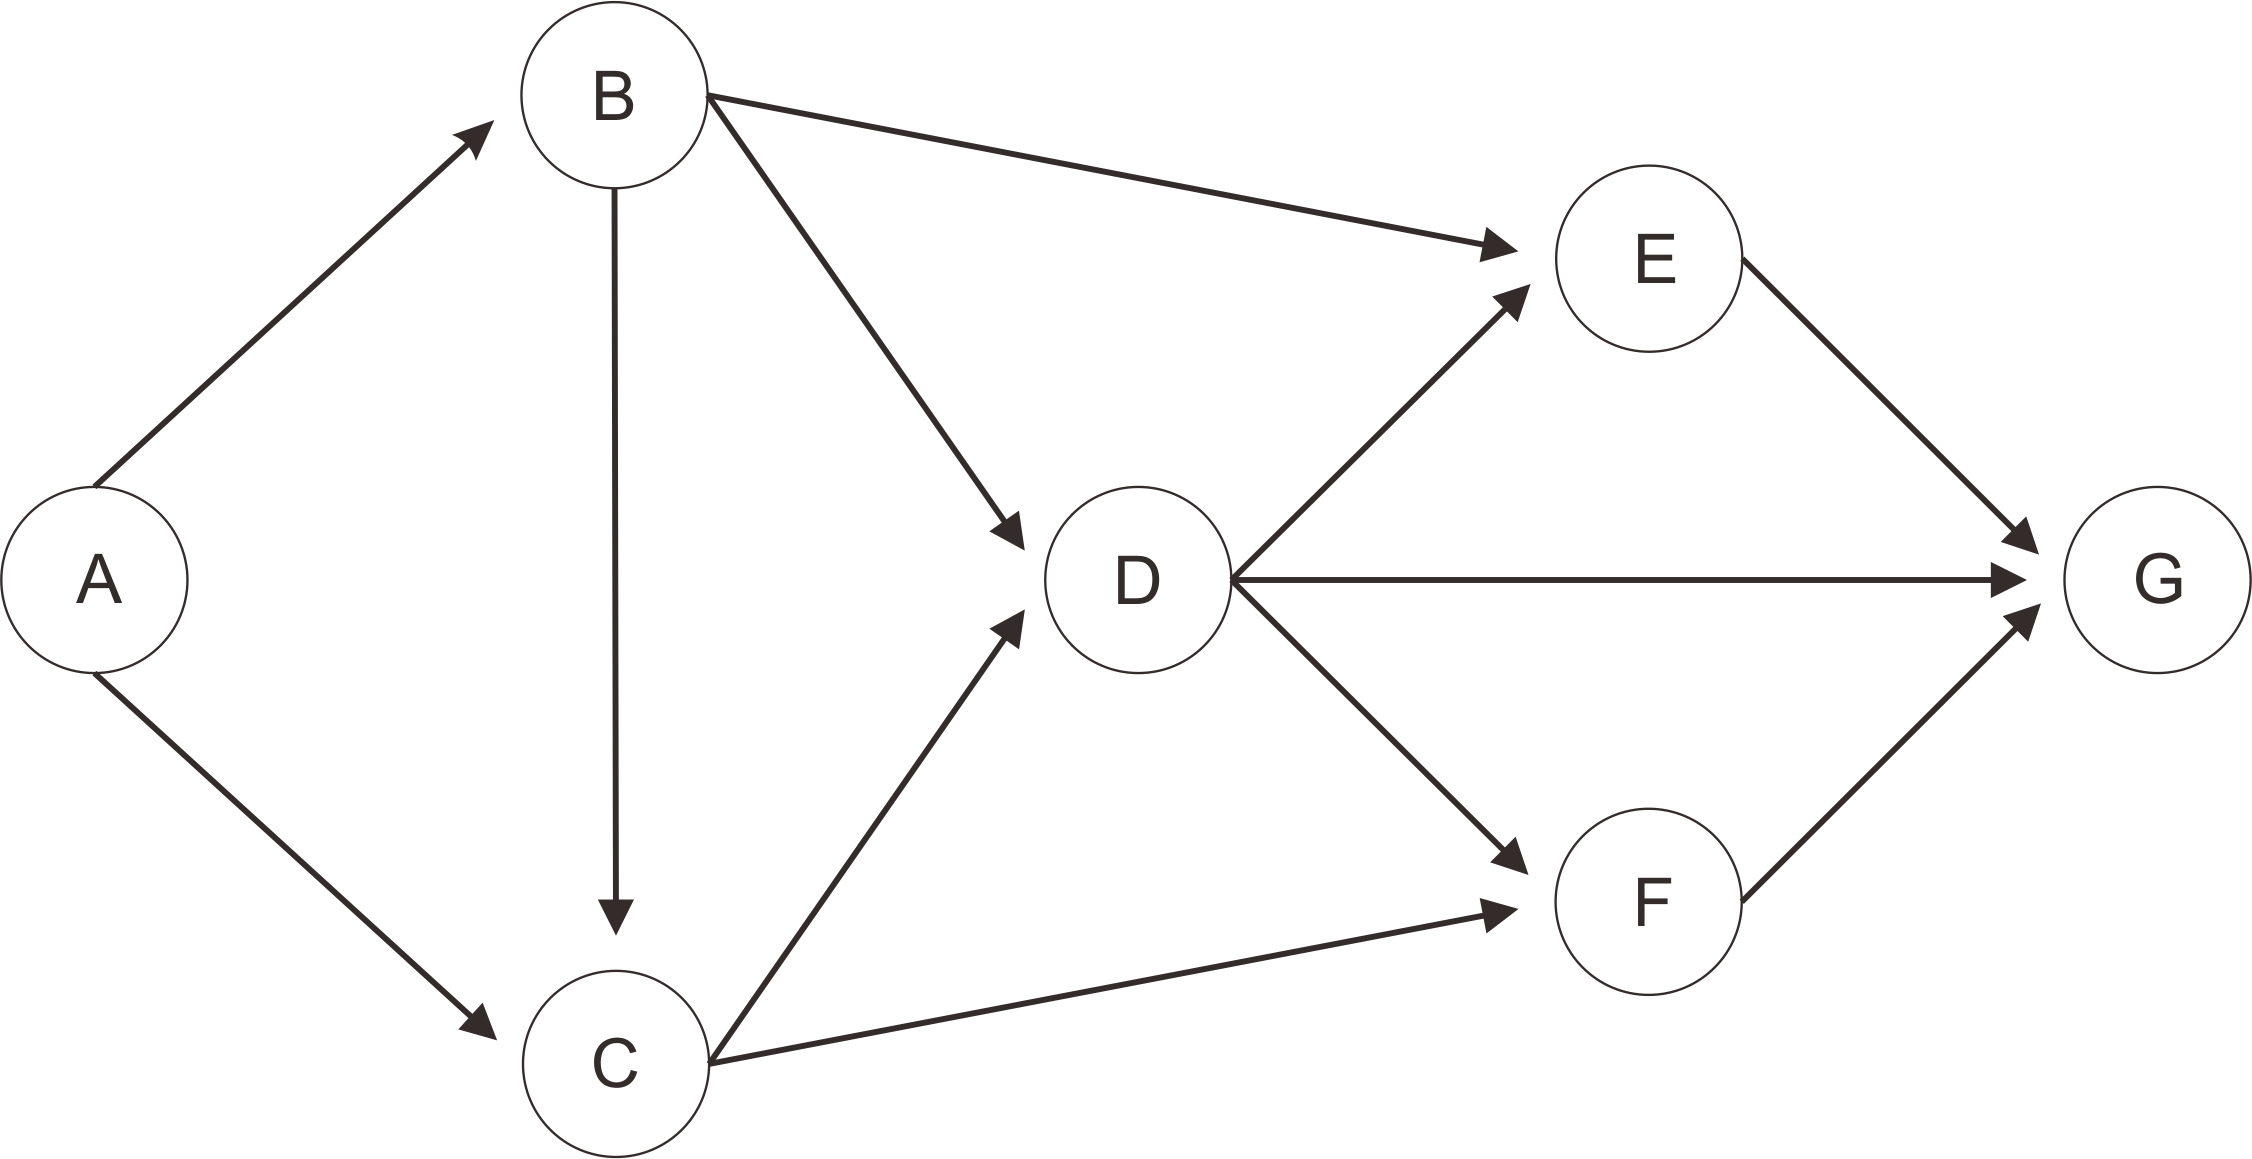
\includegraphics[scale=0.5]{graph-ABCDEFG.png}
    \caption{Graph ABCDEFG}
    \label{fig:graph-ABCDEFG}
\end{figure}

In \ref{fig:graph-ABCDEFG}, consider vertex A is the starting point and vertex G is the endpoint. To travel to vertex G there are many possible path which are :

\begin{enumerate}[leftmargin=*, topsep=5pt, itemsep=-1ex, partopsep=1ex, parsep=2ex]
\item $A \to B \to C \to D \to E \to G$ \hspace{10mm} 7. \hspace{0.5mm} $A \to B \to D \to G$
\item $A \to B \to C \to D \to F \to G$ \hspace{10mm} 8. \hspace{0.5mm} $A \to B \to E \to G$
\item $A \to B \to C \to D \to G$ \hspace{20mm} 9. \hspace{0.5mm} $A \to C \to D \to E \to G$
\item $A \to B \to C \to F \to G$ \hspace{20mm} 10. $A \to C \to D \to F \to G$
\item $A \to B \to D \to E \to G$ \hspace{20mm} 11. $A \to C \to D \to G$
\item $A \to B \to D \to F \to G$ \hspace{20mm} 12. $A \to C \to F \to G$
\end{enumerate}

Based on the above data, the shortest path can be calculated by finding the distance between the paths. If the distance between paths is not yet known, the distance can be calculated based on the coordinates of adjacent vertex.

\section{Road Network System}
Road network system is a unity of road network consisting of primary road network system and secondary road network system interwoven in hierarchy relationship. The road network system is structured with reference to the spatial plan of the region and with respect to interconnection and/or interconnection within urban areas, and rural areas \cite{zhang2005} \cite{weiping1989}.

\begin{figure}[H]
    \centering
    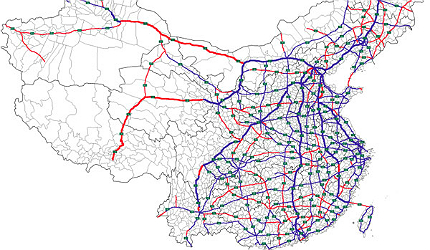
\includegraphics[scale=0.7]{road-network.jpg}
    \caption{Road Network System}
    \label{fig:Road Network System}
\end{figure}

\subsection{Road Classification}
The road is a land transport infrastructure covering all parts of the road, including auxiliary buildings and equipment intended for traffic, located on the soil surface, above ground level, below ground and / or water, and above water level, Lorries, and cable roads.

Road classification based on its function according to UU no. 38/2004 includes:
\begin{enumerate}[label=- , leftmargin=*, topsep=5pt, itemsep=-1ex, partopsep=1ex, parsep=2ex]
\item Arterial road is a public road that serves the main transport with long-distance travel features, high average speed, and the number of entrances are limited efficiently.
\item Road collector is a public road that serves to serve the collector or the spacer with medium distance features, moderate average speed, and the number of entrances is limited.
\item Local roads are public roads that serve local transport with features of short distance travel, low average speed, and unlimited number of entrances.
\item The road environment is a public road that serves the transportation of the environment with the characteristics of travel at close range, and with low average speed.
\end{enumerate}

\pagebreak

\section{K-Nearest Neighbor}
K-Nearest Neighbor (KNN) is one of classification algorithm that classifies by proximity of data with others data. In the KNN algorithm of q-dimensional data, the distance from the data to others data can be calculated. Distance values are used as proximity values or similarities between data testing and datasets. The K value of the KNN algorithm is the closest amount of data from the data testing. If K = 1, then the class of data testing is the class of the nearest neighbor. If k = 3, three closest neighbors will be taken from the dataset \cite{prasetyo2012}.

KNN is one of the most widely used algorithms in machine learning. KNN is a learning method based on the case and no learning phase is required (training). The model developed in the KNN algorithm is a training sample relating to the distance function and the choice of class function based on the nearest neighbor class. The functioning of the method depends on the choice of some number of parameters such as the K parameter representing the number of neighbors selected to assign the new data class and the distance calculation method used \cite{medjahed2013}.

\subsection{KNN Classification}
Let G is a set of a data in dataset which has class. KNN compute distance from Q to each data in dataset. Then KNN sort data with minimum distance before determine class for Q. If k=1, Q's class of data testing is the class of $g_{1}$. If k=3, Q gets three closest neighbors which is $g_{1}$, $g_{2}$, and $g_{3}$.

\begin{figure}[H]
    \centering
    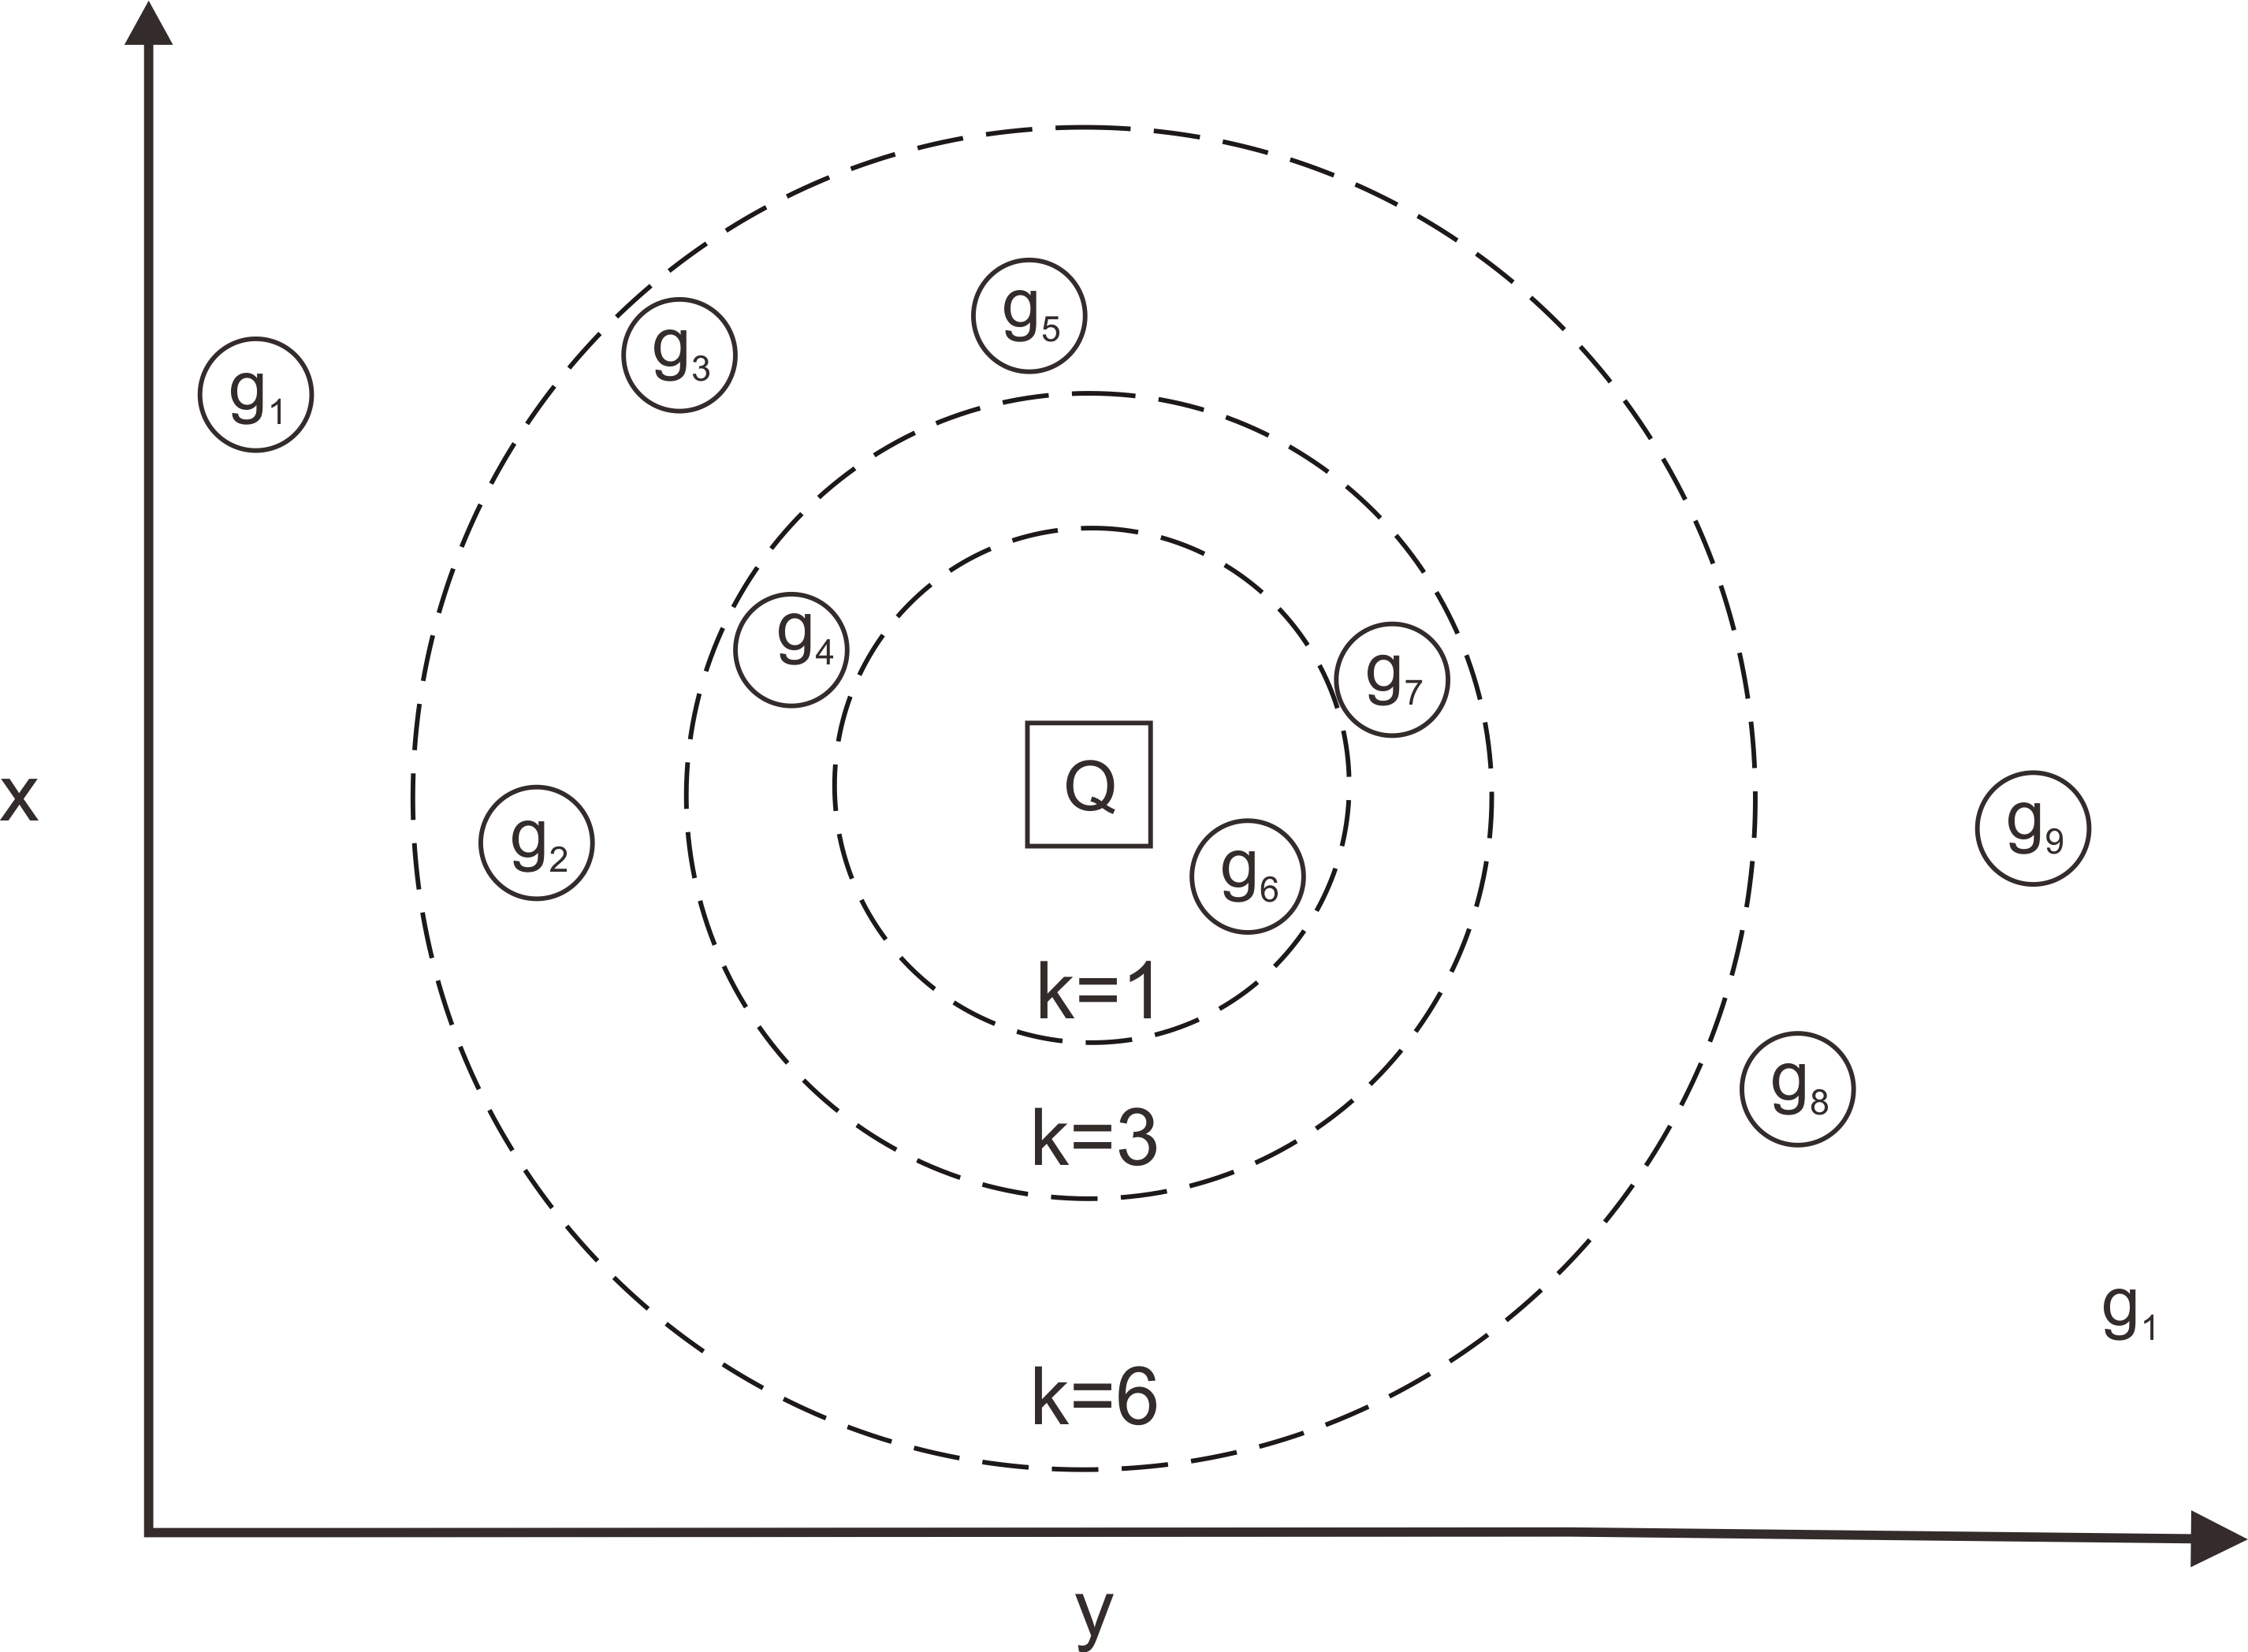
\includegraphics[scale=0.4]{knn.png}
    \caption{K-Nearest Neighbor}
    \label{fig:KNN}
\end{figure}



\subsection{Advantages and Disadvantages from KNN}
KNN algorithm has several advantages including KNN algorithm is a simple classification algorithm, the resilience of dataset interference, and effectiveness in the dataset adequate. However, the KNN algorithm also has disadvantages as follows \cite{zhang2013} :

\begin{enumerate}[label=- , leftmargin=*, topsep=5pt, itemsep=-1ex, partopsep=1ex, parsep=2ex]
\item KNN algorithm has a high computational cost. To determine the nearest k-neighbor of a data testing, all similarities between the data testing and the dataset must be calculated.
\item KNN algorithm has a dependency on the dataset. The resulting classification is only based on the sample dataset and does not use any additional data. This makes the KNN algorithm highly dependent on the dataset.
\item KNN algorithm also has weaknesses in terms of low accuracy in multidimensional data sets, K parameters, and distance calculation methods.
\end{enumerate}


\section{Voronoi Diagram}
The Voronoi Diagram has been applied to many location problems \cite{okabe2000}. The Voronoi diagram is data structure extensively in the domain of computatuional geometry. Originally, it characetrizes regions of proximity for a set of $k$ sites in the plane where distance poinrs is defined by their Euclidean distance. Optimal algortihms exist to compute the Voronoi diagram in $0(k log k)$ time, and the Voronoi diagram can be represented in $0(k)$ space \cite{erwig2000}.

\begin{figure}[H]
    \centering
    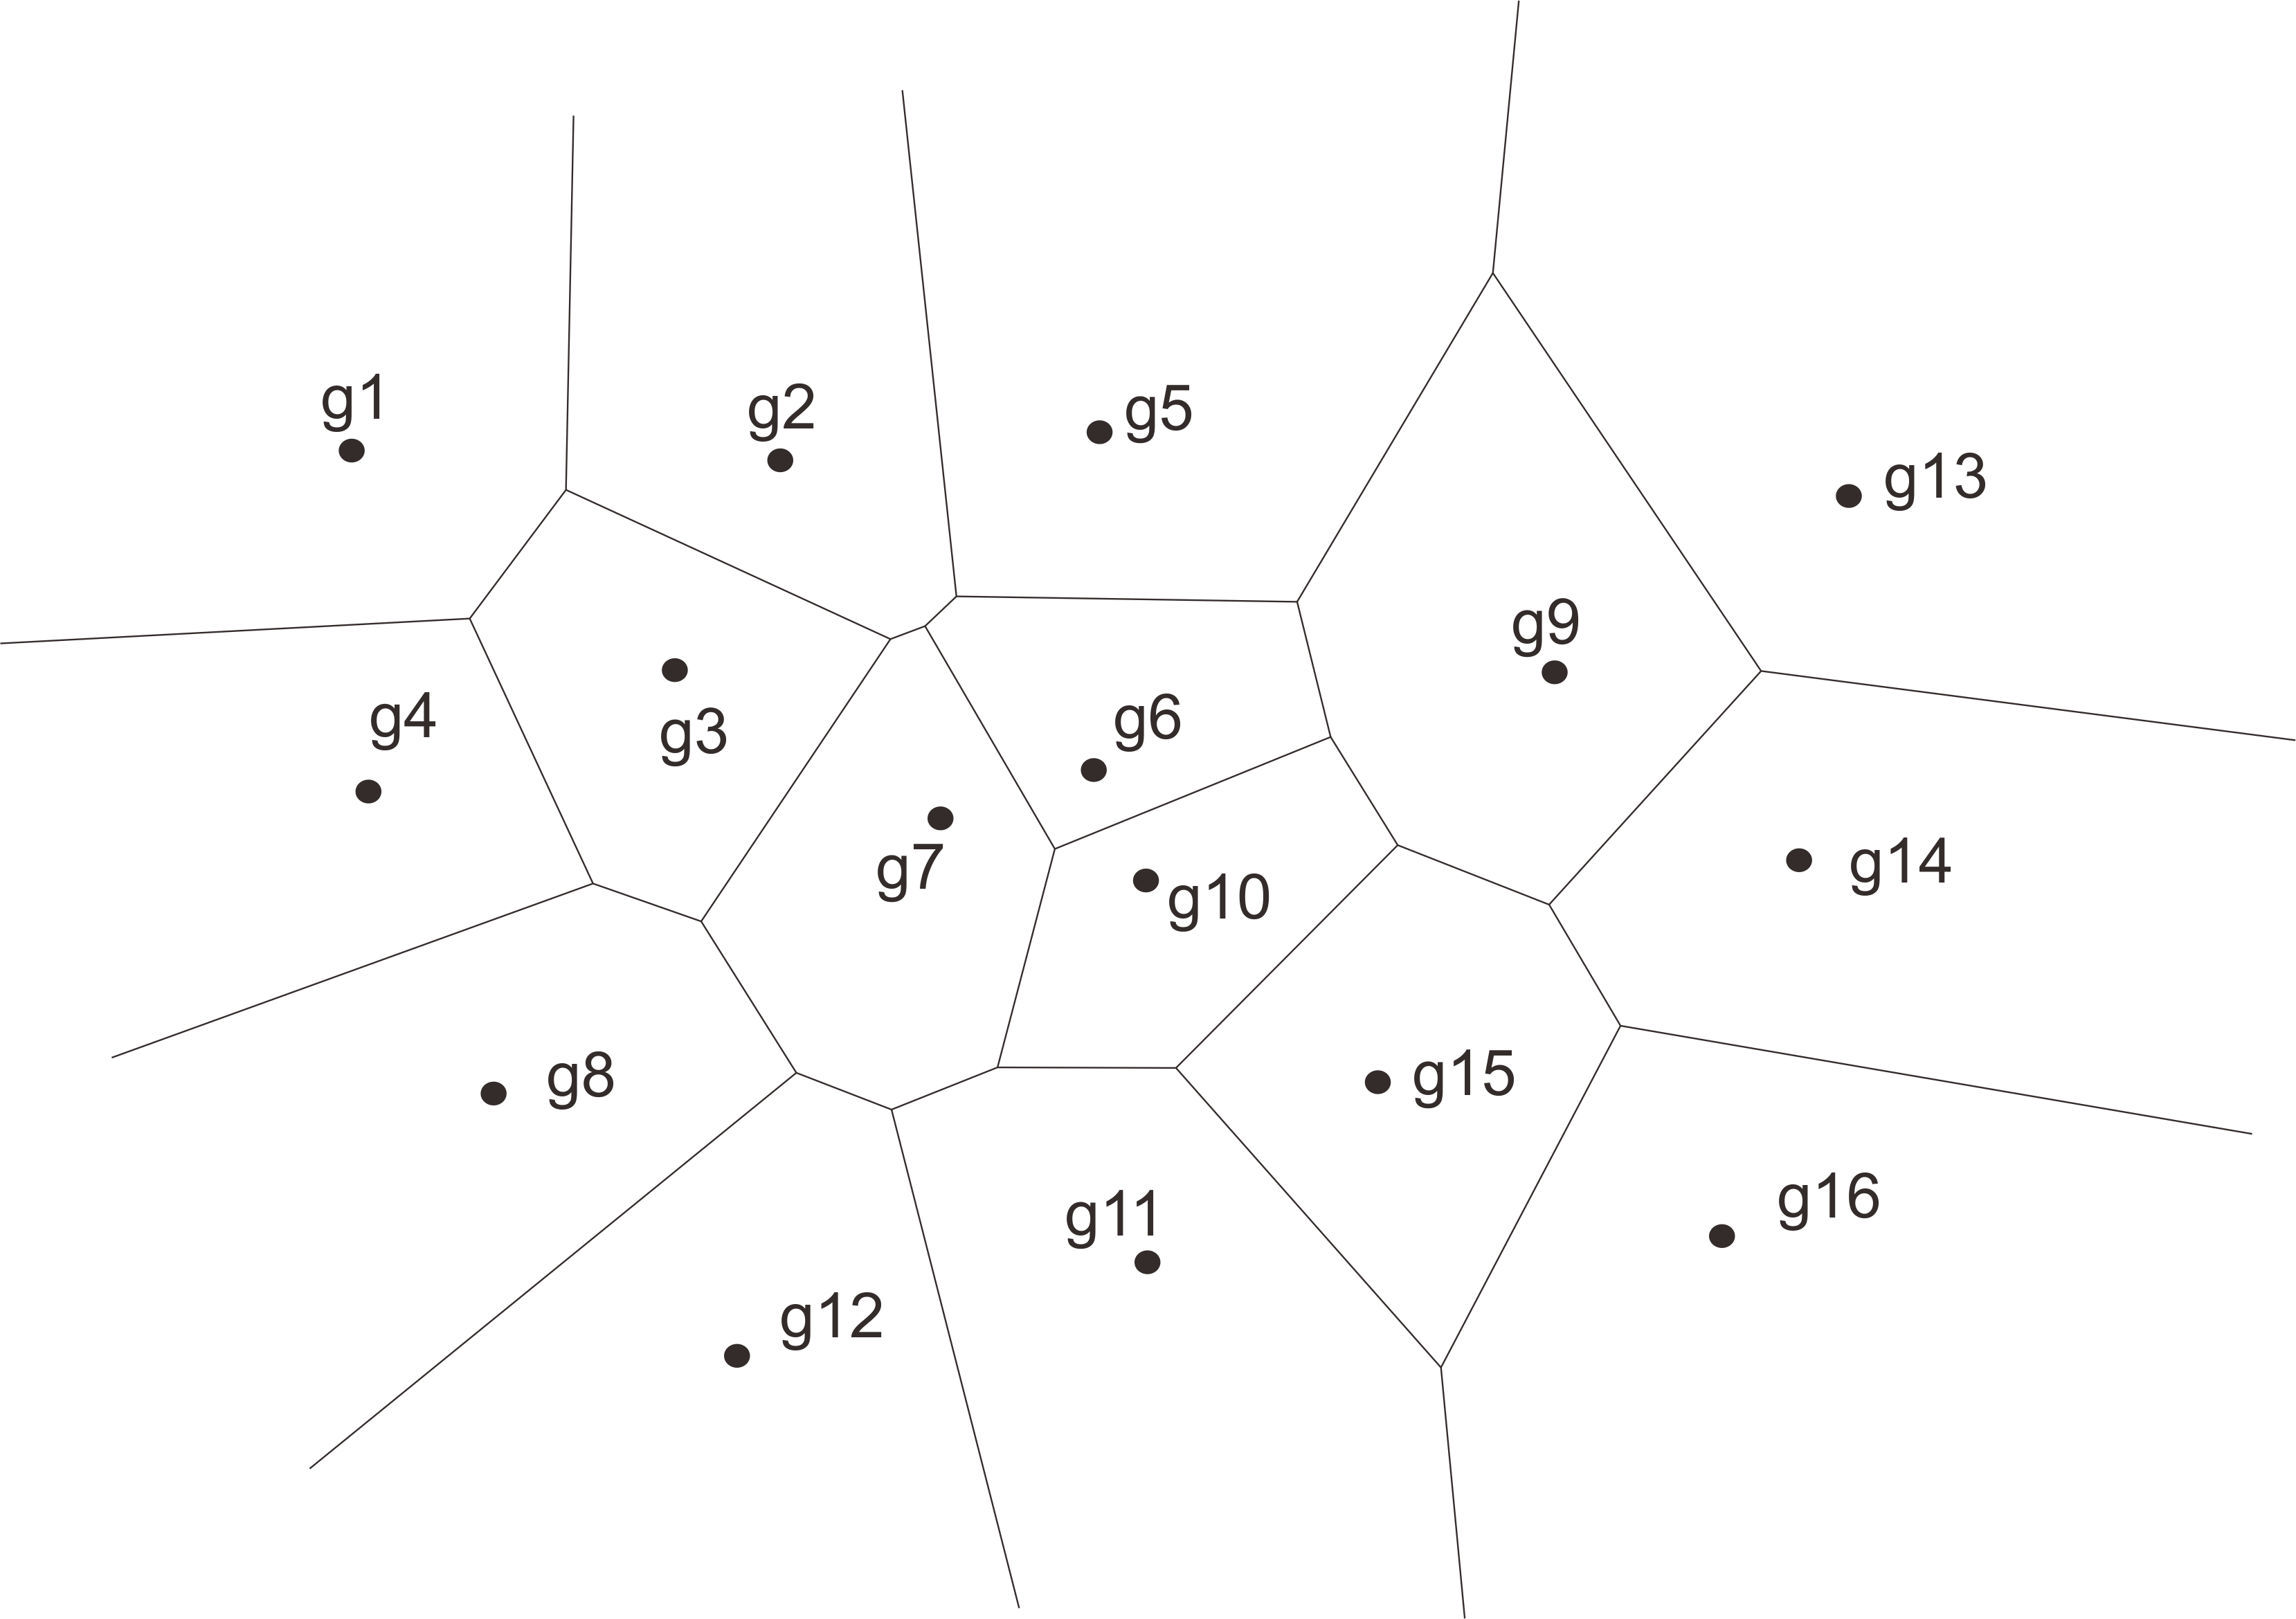
\includegraphics[scale=0.4]{voronoi-diagram.png}
    \caption{Voronoi Diagram}
    \label{fig:my_label}
\end{figure}

For example there is a set point generator on Euclidean field (in general, the generator can be any type of spatial objects). Consider all locations in the area has been associate for their closest generator. Set the location assigned to each generator forming region called Voronoi cell. This Voronoi Cell basically based of it generator. More specifically, Voronoi polygon formed by dividing border point which is the middle point betweens the generator with it adjacent generators. Set of Voronoi polygon formed is called a Voronoi diagram.

There are 4 review from basic geometric properties of the Voronoi diagrams as follows \cite{kolah2004} :
\begin{enumerate}[label=- , leftmargin=*, topsep=5pt, itemsep=-1ex, partopsep=1ex, parsep=2ex]
	\item Property 1: The Voronoi diagram of a point set $G$, $VD(G)$, is unique.
	\item Property 2: The nearest generator point of $g_{i}$ (e.g., $g_{j}$) is among the generator points whose Voronoi polygons share similar Voronoi edges with V P(pi).
	\item Property 3: Let $n$ and $n_{e}$ be the number of generator points and Voronoi edges, respectively, then $n_{e} \leq 3n - 6$.
	\item Property 4: From property 3, and the fact that every Voronoi edge is shared by exactly two Voronoi polygons, notice that the average number of Voronoi edges per Voronoi polygon is at most 6, i.e., $2(3n-6)/n = 6/12n \leq 6$. This means that on average, each generator has 6 adjacent generators.
\end{enumerate}



\section{Network Voronoi Diagram}
Voronoi diagram in the plane is sometimes inadequate for the location problem \cite{takehiro2005}. The reason is that the distances can not be measured by the Euclidean distances in some problems. So there’s a network and defined by nodes and arcs which is the partition of the two.

\begin{figure}[H]
    \centering
    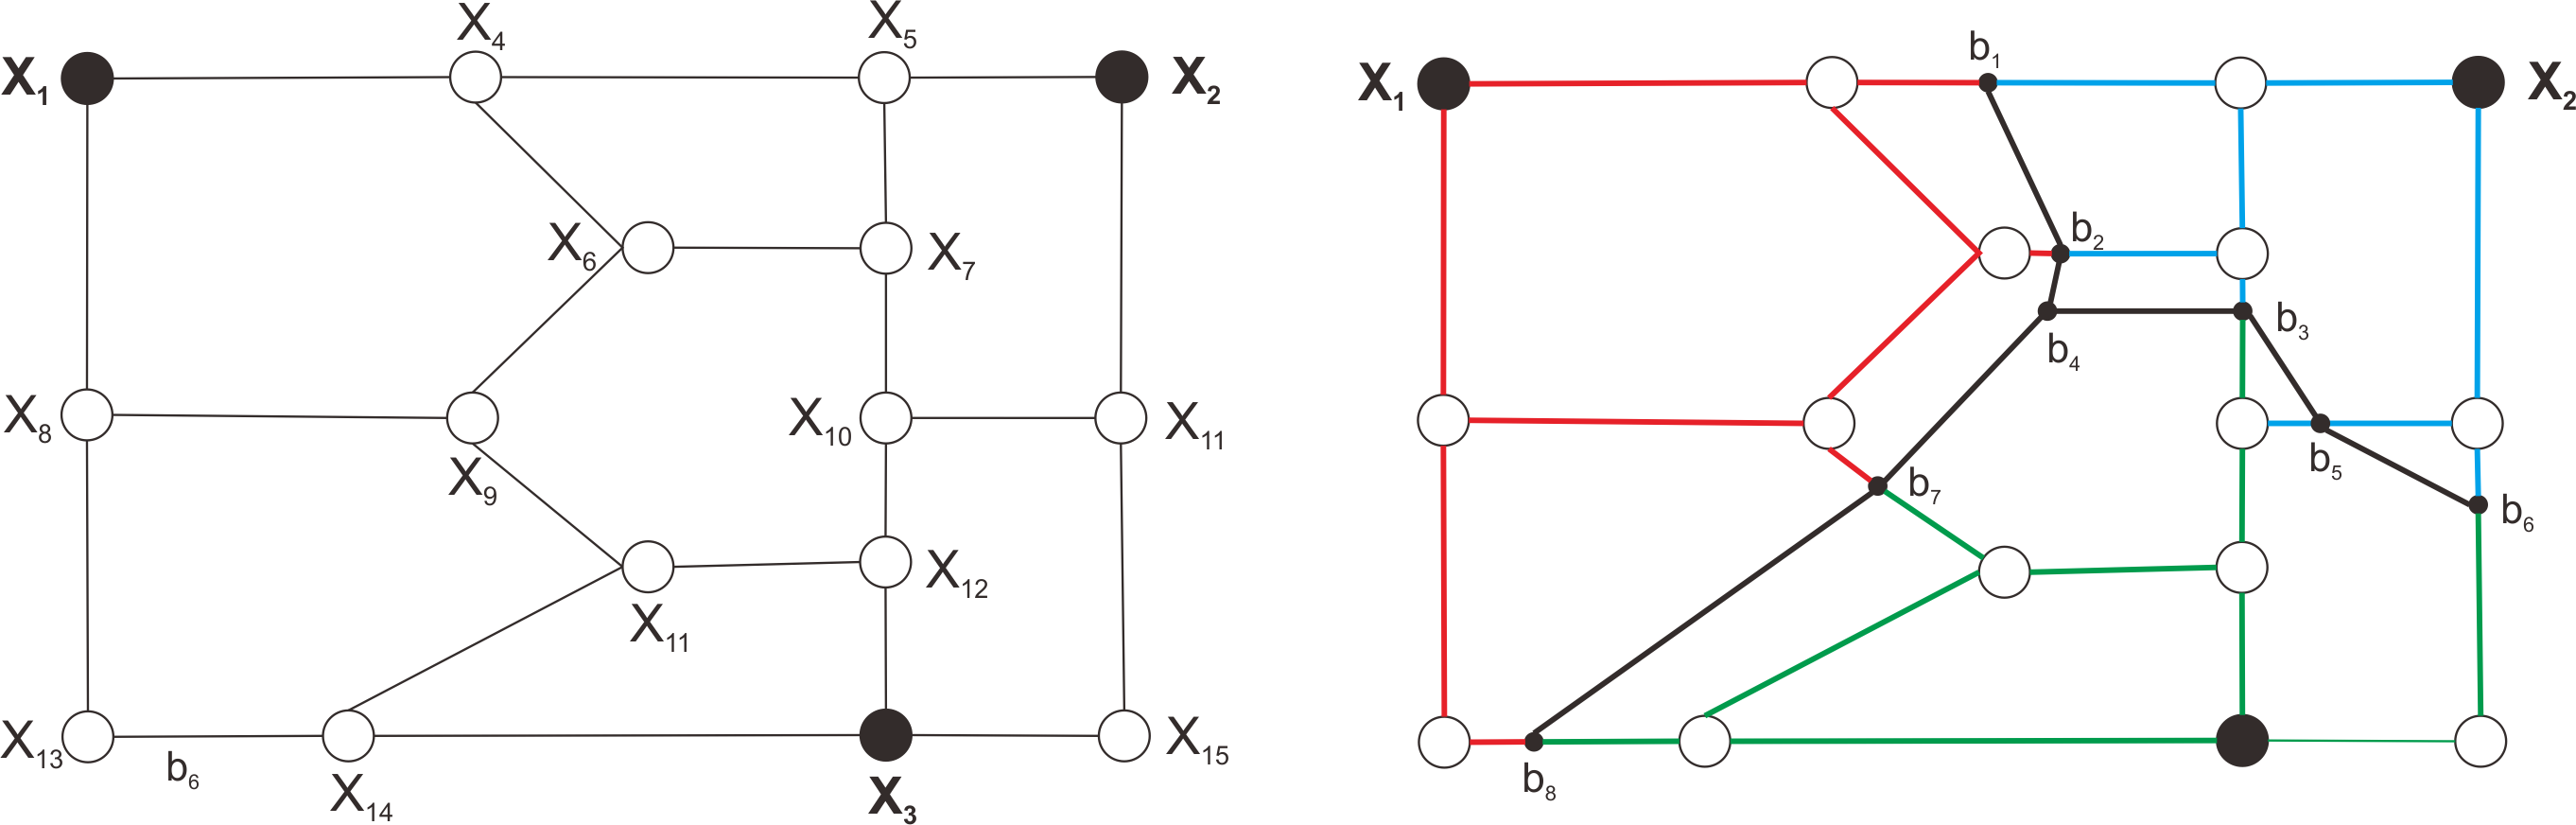
\includegraphics[scale=0.6]{network-voronoi-diagram.png}
    \caption{Network Voronoi Diagram}
    \label{fig:my_label}
\end{figure}    
    
\pagebreak
Network Voronoi diagram is based on Djikstra's algorithm calculates in  a connected network \cite{erwig2000}. NVD is defined by consider a network $N(V, E)$ and a set of vertices $V = {x_{1}, x_{n}, x_{n+1} ..., x_{o}} \subseteq V$, where the first $n$ elements (ie., $G = {g_{1}, ..., g_{n}}$) are the generators (e.g., points of interest in road network). Each edge in $N(V, E)$ has positive length. All vertices that are closer to $g_{i}$ represent $g_{i}$ dominance over its adjacent generator. The set $b(g_{i}, g{j})$, called border points between $g_{i}$ and $g_{j}$, specifies all points in all edge that are equally distance from $g_{i}$ and $g_{j}$.

The algorithm for computing the Network Voronoi Diagram is shown in the following pseudocode.

\begin{algorithm}
\caption{Network Voronoi Diagram Algorithm}
\begin{algorithmic}[1]
\Procedure{constructNVD}{}
\ForEach {$v \in S$}:
	\If{$v \in G$}
		\State $V(v)\gets g$
		\State $d(v)\gets 0$
		\State $insert(v)$
	\Else
		\State $V(v)\gets null$
		\State $d(v)\gets \infty$
	\EndIf
\EndFor

\While{$Queue\not=empty$}
	\State $v_{min}\gets extractmin()$
	\State mark  $v$
	\ForEach{$neighbor(v, w)$ with $w$ not marked}
		\State $\Delta\gets d(v_{min}) + l(v, w)$
		\If{$d(w) = \infty$}
			\State $d(w)\gets \Delta$
			\State $V(w)\gets V(v_{min})$
			\State $insert(w)$
		\Else
			\State $V(w)\gets V(v)$
			\State $decreaseKey(w, \delta)$
		\EndIf
	\EndFor
\EndWhile
\EndProcedure
\end{algorithmic}
\end{algorithm}

\pagebreak
\section{K-Nearest Neighbor in Network Voronoi Diagram} 

The k-nearest neighbor Voronoi diagram has also important uses in computation geometry and in location problems. Given the set of the generator g in a space S and query point QP. Let d(g) denotes distance g to QP. For each g, d(g) will be computed and store it at queue. After that, queue being sorted by minimum distance. So by looking into queue order k-nearest generator will be found.
\begin{figure}[H]
    \centering
    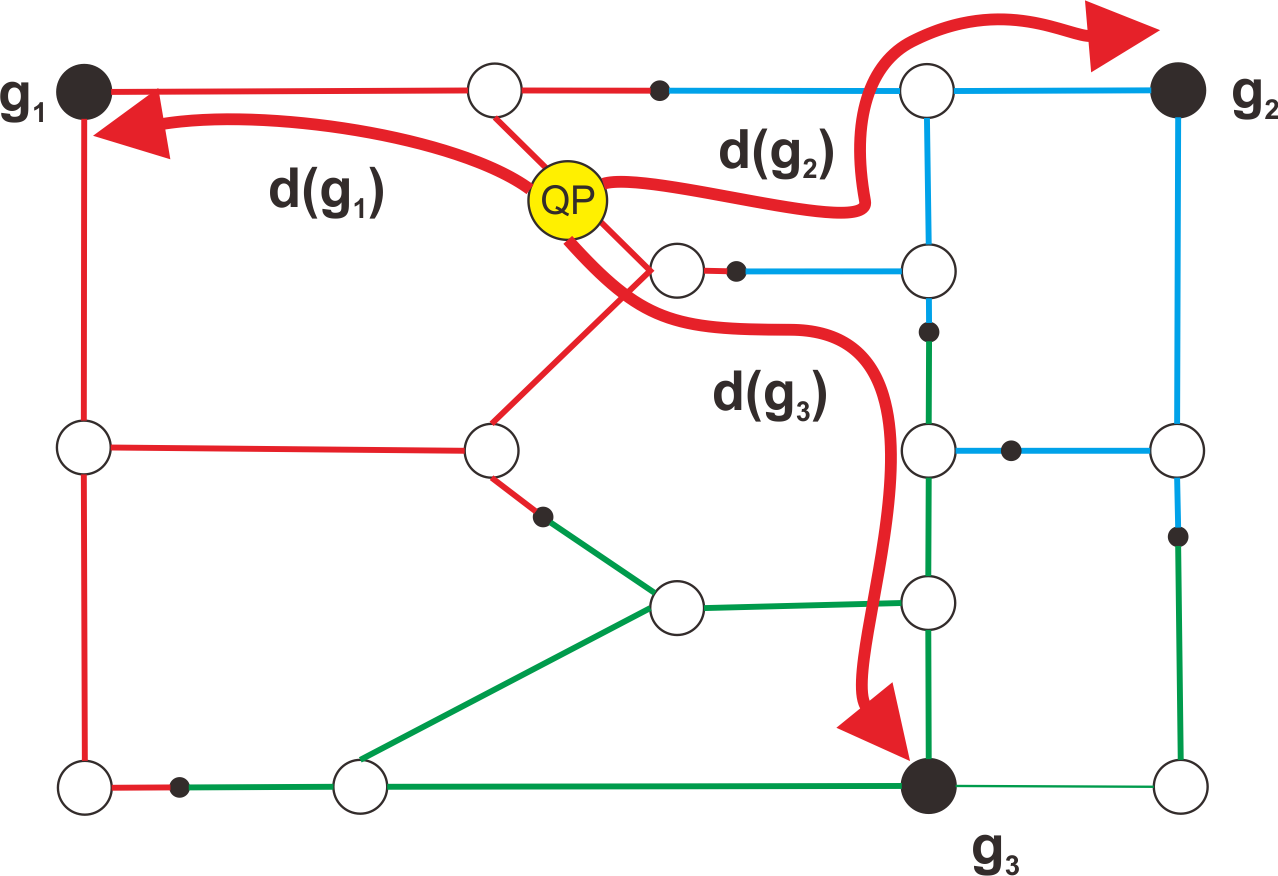
\includegraphics[scale=0.8]{knn_basic.png}
    \caption{KNN algorithm in road network}
    \label{fig:my_label}
\end{figure} 

The algorithm for computing the K-Nearest Neighbor in Network Voronoi Diagram is shown in the following pseudocode.

\begin{algorithm}
\caption{Basic KNN Algorithm in NVD}
\begin{algorithmic}[1]
\Function{KNN($QP$, $k$)}{}
\ForEach {$g \in S$}:
	\State $d(g) \gets count_distance(g, QO)$
	\State $insert(g)$
\EndFor
\State $sort Queue by minimum d$
\Return $Queue[k]$
\EndFunction
\end{algorithmic}
\end{algorithm}
